% !TEX root = ..\thesis.tex

\chapter{ Mô hình}
% vẽ sơ đồ hệ thống

Mô hình tổng quan của đề tài hình \ref{fig:general_chart}
\begin{figure}[H]
    \centering
    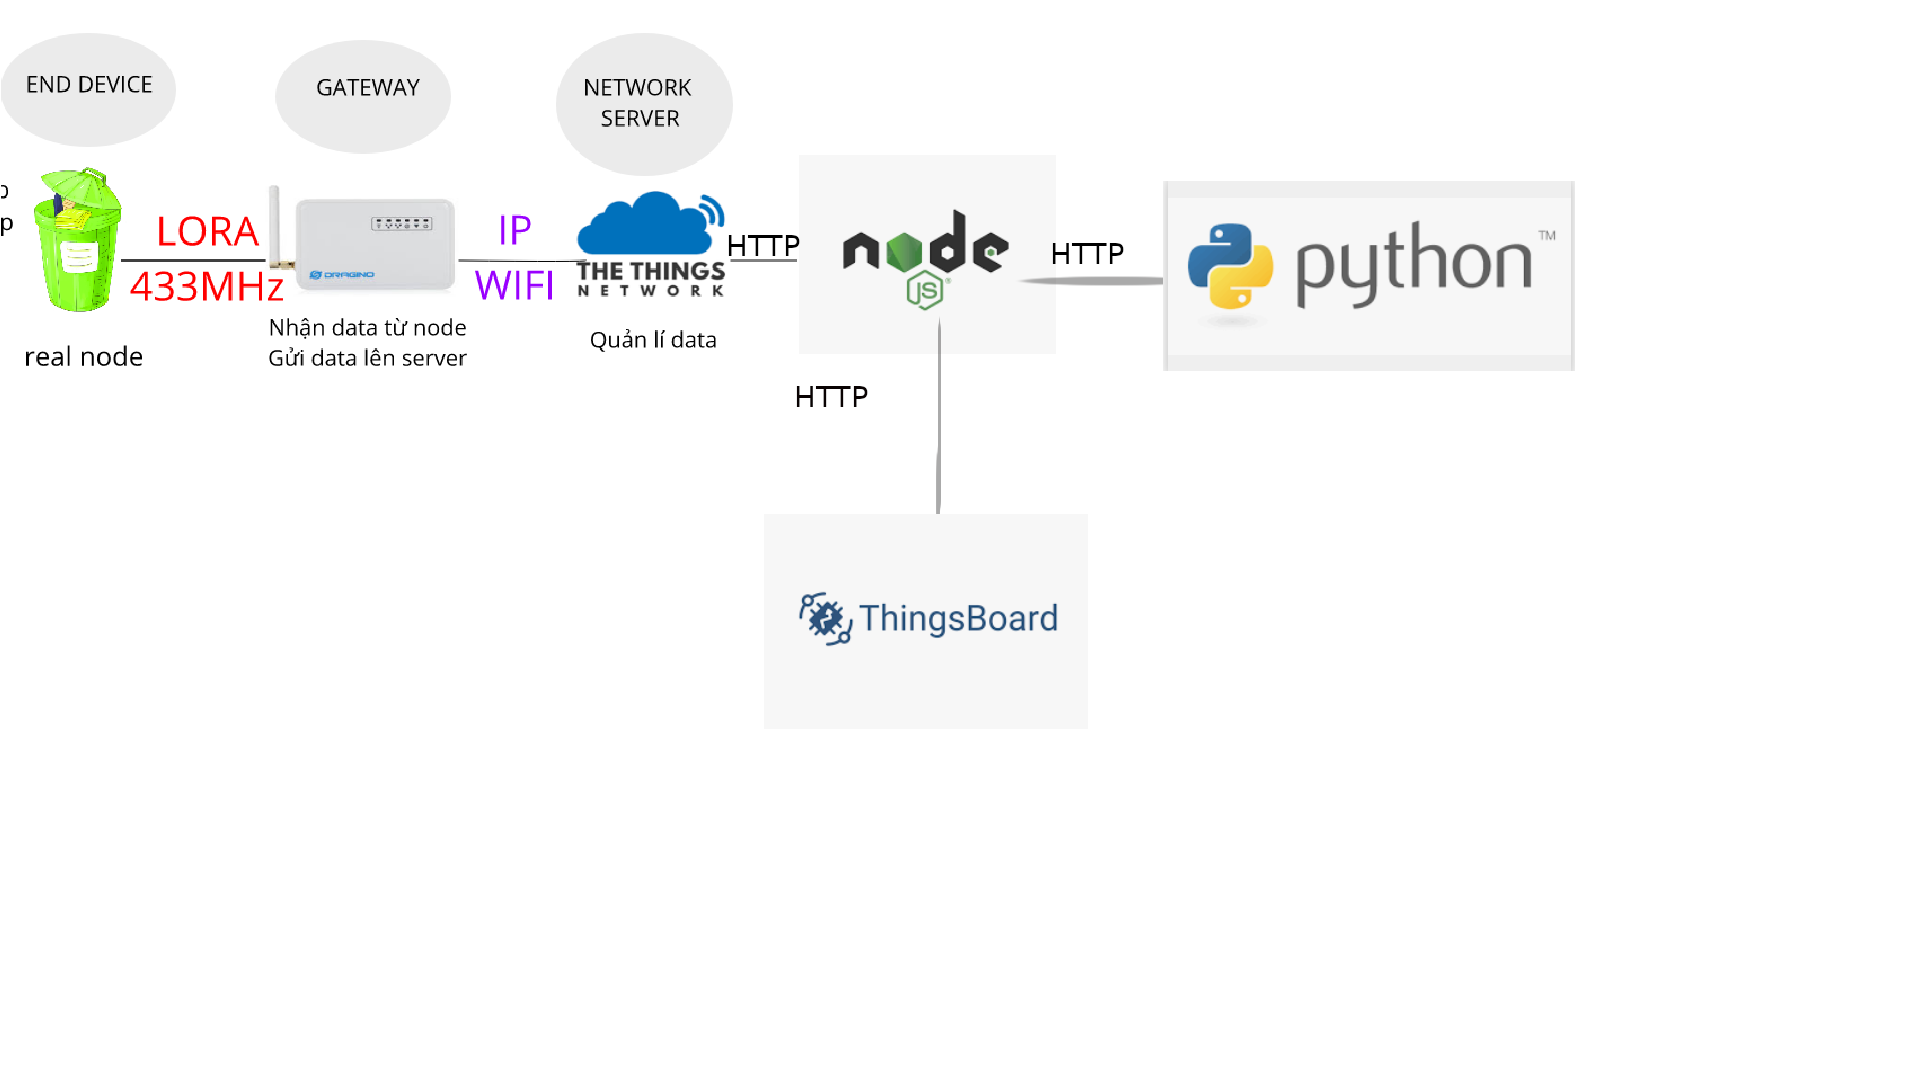
\includegraphics[width=\textwidth]{images/Quanh/general_chart.png}
    \caption{Mô hình tổng quan}
    \label{fig:general_chart}
\end{figure}
Ở mô hình tổng quan đề tài, chúng tôi chia làm 2 phần, về thiết bị và về server.

\begin{itemize}
    \item Về thiết bị, tôi gắn 2 loại board và 2 ultrasonic sensor vào thùng rác để thực hiện 2 mục đích khác nhau, cụ thể:
        \begin{itemize}
            \item ESP32 camera AI Thinker, dùng vào mục đích chụp ảnh và phục vụ chức năng phân loại rác thải.
            \item  ESP32 Lora heltec, dùng trong mục đích thu thập data và gửi data cho server bằng công nghệ LoRaWAN.
            \item Ultrasonic sensor thực hiện nhiệm vụ đo độ dài khoảng trống còn lại trong thùng rác.
        \end{itemize}

    \item Về server, sử dụng Nodejs và Flask làm server cung cấp API, Thingsboard để làm giao diện hiển thị và một số server thứ ba khác, chức năng được mô tả cụ thể như sau:
        \begin{itemize}
            \item Nodejs Server là server nhận và xử lý chính dữ liệu, lưu trữ dữ liệu cho từng thùng rác. Từ đó, sử dụng dữ liệu để hiển thị, dự đoán và tìm đường đi tối ưu nhất để thu gom rác.
            \item Flask Server là server sử dụng Deep Learning để dự đoán dữ liệu được gửi từ Nodejs Server.
            \item Thingsboard là giao diện lưu trữ thông tin thùng rác, hiển thị dữ liệu theo nhiều dạng và vẽ đường đi trên bản đồ.
            \item Ngoài ra, còn sử dụng Thingsboard server hỗ trợ API thao tác đến Thingsboard và Mapbox server hỗ trợ API liên quan đến địa lý và đường đi.
        \end{itemize}
   

\end{itemize}


Hình \ref{fig:chart_smartbin} mô tả chi tiết về cấu tạo của thùng rác, và các thức hoạt động của 2 loại board được gắn bên trong thùng. 
\begin{figure}[H]
    \centering
    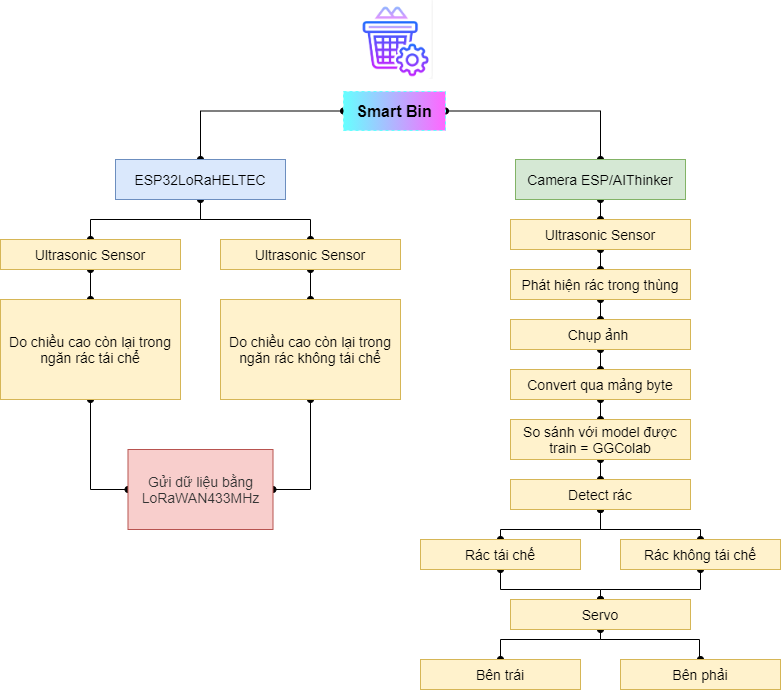
\includegraphics[width=\textwidth]{images/Chart_smartbin.png}
    \caption{Mô hình device}
    \label{fig:chart_smartbin}
\end{figure}


Mô hình server từ bước khởi tạo đến gửi dữ liệu \ref{fig:chart_server1}
\begin{figure}[H]
    \centering
    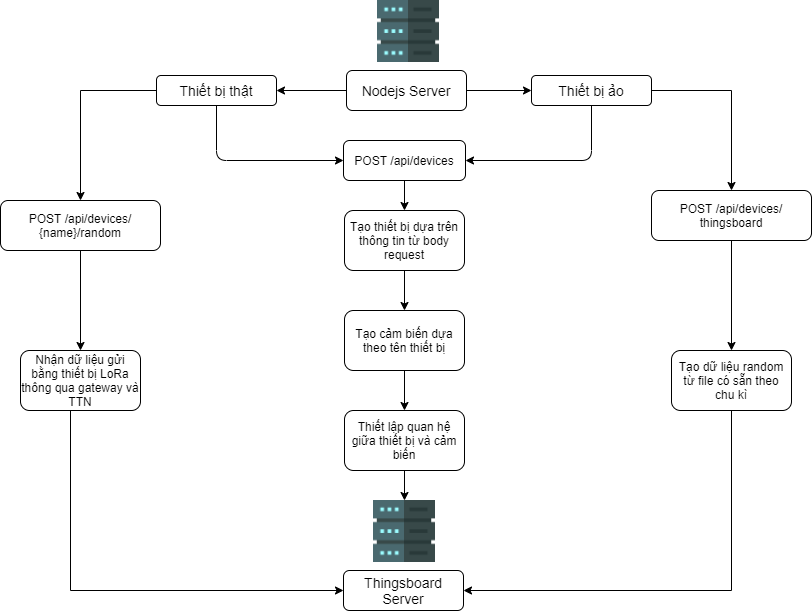
\includegraphics[width=\textwidth]{images/Khanh/Nodejs/Chart_server1.png}
    \caption{Mô hình server từ bước khởi tạo đến gửi dữ liệu}
    \label{fig:chart_server1}
\end{figure}

Mô hình server từ bước gửi dữ liệu đến xử lý bản đồ \ref{fig:chart_server2}
\begin{figure}[H]
    \centering
    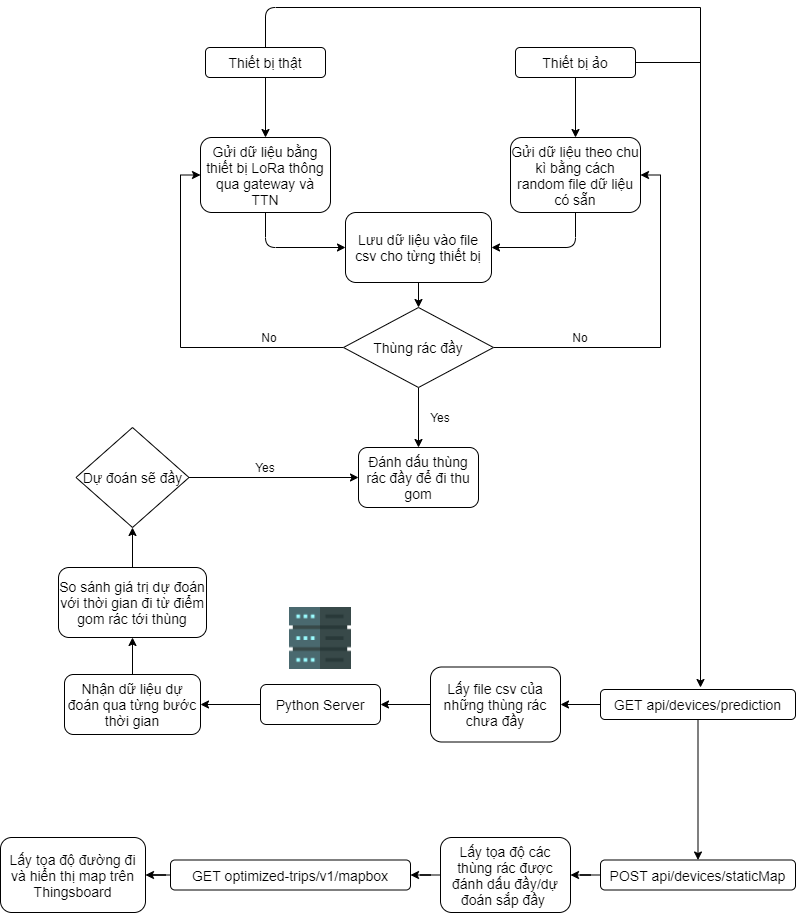
\includegraphics[width=\textwidth]{images/Khanh/Nodejs/Chart_server2.png}
    \caption{Mô hình server từ bước gửi dữ liệu đến xử lý bản đồ}
    \label{fig:chart_server2}
\end{figure}